% Hlavicka pro protokoly z fyzikalniho praktika.
% Verze pro: LaTeX
% Verze hlavicky: 22. 2. 2007
% Autor: Ustav fyziky kondenzovanych latek
% Ke stazeni: www.physics.muni.cz/ufkl/Vyuka/
% Licence: volne k pouziti, nejlepe k vcasnemu odevzdani protokolu z Vaseho mereni.


\documentclass[czech,11pt,a4paper]{article}
\usepackage[T1]{fontenc}
\usepackage{graphicx, animate}
\usepackage{mathtools}
\usepackage{amssymb}
\usepackage{amsthm}
\usepackage{thmtools}
\usepackage{xcolor}
\usepackage{nameref}
\usepackage{babel}
\usepackage{hyperref}
\usepackage{multicol}
\usepackage[export]{adjustbox}
\usepackage{subcaption}
\usepackage{caption}
\usepackage{multirow}
\usepackage{float}
\usepackage{placeins}
\usepackage{biblatex}
\graphicspath{ {./images/} }




%%% Nemente:
\usepackage[margin=2cm]{geometry}
\newtoks\jmenopraktika \newtoks\jmeno \newtoks\datum
\newtoks\obor \newtoks\skupina \newtoks\rocnik \newtoks\semestr
\newtoks\cisloulohy \newtoks\jmenoulohy

%%% Nemente - konec.


%%%%%%%%%%% Doplnte pozadovane polozky:

\jmenopraktika={Fyzikální praktikum 3}  % nahradte jmenem vaseho predmetu
\jmeno={Teodor Duraković}            % nahradte jmenem mericiho
\datum={18.~března 2024}        % nahradte datem mereni ulohy
\obor={F}                     % nahradte zkratkou vami studovaneho oboru
\skupina={Út 14:00}            % nahradte dobou vyuky vasi seminarni skupiny
\rocnik={II}                  % nahradte rocnikem, ve kterem studujete
\semestr={IV}                 % nahradte semestrem, ve kterem studujete

\cisloulohy={6}               % nahradte cislem merene ulohy
\jmenoulohy={Zeemanův jev}           % nahradte vlhkosti vzduchu pri mereni (v %)

%%%%%%%%%%% Konec pozadovanych polozek.


%%%%%%%%%%% Uzitecne balicky:

%%%%%% Zamezeni parchantu:
\widowpenalty 10000 \clubpenalty 10000 \displaywidowpenalty 10000
%%%%%% Parametry pro moznost vsazeni vetsiho poctu obrazku na stranku
\setcounter{topnumber}{3}	  % max. pocet floatu nahore (specifikace t)
\setcounter{bottomnumber}{3}	  % max. pocet floatu dole (specifikace b)
\setcounter{totalnumber}{6}	  % max. pocet floatu na strance celkem
\renewcommand\topfraction{0.9}	  % max podil stranky pro floaty nahore
\renewcommand\bottomfraction{0.9} % max podil stranky pro floaty dole
\renewcommand\textfraction{0.1}	  % min podil stranky, ktery musi obsahovat text
\intextsep=8mm \textfloatsep=8mm  %\intextsep pro ulozeni [h] floatu a \textfloatsep pro [b] or [t]

% Tecky za cisly sekci:
\renewcommand{\thesection}{\arabic{section}.}
\renewcommand{\thesubsection}{\thesection\arabic{subsection}.}
\renewcommand{\thesubsubsection}{\thesubsection\arabic{subsubsection}.}
% Jednopismenna mezera mezi cislem a nazvem kapitoly:
\makeatletter \def\@seccntformat#1{\csname the#1\endcsname\hspace{1ex}} \makeatother


%%%%%%%%%%%%%%%%%%%%%%%%%%%%%%%%%%%%%%%%%%%%%%%%%%%%%%%%%%%%%%%%%%%%%%%%%%%%%%%
%%%%%%%%%%%%%%%%%%%%%%%%%%%%%%%%%%%%%%%%%%%%%%%%%%%%%%%%%%%%%%%%%%%%%%%%%%%%%%%
% Zacatek dokumentu
%%%%%%%%%%%%%%%%%%%%%%%%%%%%%%%%%%%%%%%%%%%%%%%%%%%%%%%%%%%%%%%%%%%%%%%%%%%%%%%
%%%%%%%%%%%%%%%%%%%%%%%%%%%%%%%%%%%%%%%%%%%%%%%%%%%%%%%%%%%%%%%%%%%%%%%%%%%%%%%

\begin{document}
	
	%%%%%%%%%%%%%%%%%%%%%%%%%%%%%%%%%%%%%%%%%%%%%%%%%%%%%%%%%%%%%%%%%%%%%%%%%%%%%%%
	% Nemente:
	%%%%%%%%%%%%%%%%%%%%%%%%%%%%%%%%%%%%%%%%%%%%%%%%%%%%%%%%%%%%%%%%%%%%%%%%%%%%%%%
	\thispagestyle{empty}
	
	{
		\begin{center}
			\sf 
			{\Large Ústav fyziky a technologií plazmatu Přírodovědecké fakulty Masarykovy univerzity} \\
			\bigskip
			{\huge \bfseries FYZIKÁLNÍ PRAKTIKUM} \\
			\bigskip
			{\Large \the\jmenopraktika}
		\end{center}
		
		\bigskip
		
		\sf
		\noindent
		\setlength{\arrayrulewidth}{1pt}
		\begin{tabular*}{\textwidth}{@{\extracolsep{\fill}} l l}
			\large {\bfseries Zpracoval:}  \the\jmeno & \large  {\bfseries Naměřeno:} \the\datum\\[2mm]
			\large  {\bfseries Obor:} \the\obor  \hspace{40mm}  {\bfseries Skupina:} \the\skupina %
			%{\bfseries Ročník:} \the\rocnik \hspace{5mm} {\bfseries Semestr:} \the\semestr  
			&\large {\bfseries Testováno:}\\
			\\
			\hline
		\end{tabular*}
	}
	
	\bigskip
	
	{
		\sf
		\noindent \begin{tabular}{p{3cm} p{0.6\textwidth}}
			\Large  Úloha č. {\bfseries \the\cisloulohy:} \par
			\smallskip
			&\Large \bfseries \the\jmenoulohy  \\[2mm]
		\end{tabular}
	}
	
	\vskip1cm
	
	%%%%%%%%%%%%%%%%%%%%%%%%%%%%%%%%%%%%%%%%%%%%%%%%%%%%%%%%%%%%%%%%%%%%%%%%%%%%%%%
	% konec Nemente.
	%%%%%%%%%%%%%%%%%%%%%%%%%%%%%%%%%%%%%%%%%%%%%%%%%%%%%%%%%%%%%%%%%%%%%%%%%%%%%%%
	
	%%%%%%%%%%%%%%%%%%%%%%%%%%%%%%%%%%%%%%%%%%%%%%%%%%%%%%%%%%%%%%%%%%%%%%%%%%%%%%%
	%%%%%%%%%%%%%%%%%%%%%%%%%%%%%%%%%%%%%%%%%%%%%%%%%%%%%%%%%%%%%%%%%%%%%%%%%%%%%%%
	% Zacatek textu vlastniho protokolu
	%%%%%%%%%%%%%%%%%%%%%%%%%%%%%%%%%%%%%%%%%%%%%%%%%%%%%%%%%%%%%%%%%%%%%%%%%%%%%%%
	%%%%%%%%%%%%%%%%%%%%%%%%%%%%%%%%%%%%%%%%%%%%%%%%%%%%%%%%%%%%%%%%%%%%%%%%%%%%%%%
	
	\begin{multicols}{2}
		\section{Zadání}
	
1. Ověřte funkci Fabry-Perotova interferometru. Ukažte, že naměřené poloměry různých interferenčních kroužků jedné vlnové délky souhlasí s vhodným vztahem uvedeným v návodu. \\
2. Pomocí posunu vlnočtů při normálním Zeemanově jevu zjistěte velikost Bohrova magnetonu.\\
3. Zjistěte, které složky rozštěpených spektrálních čar jsou vyzařovány ve směru kolmém na indukci magnetického pole, a které ve směru rovnoběžném. Změřte, jak jsou jednotlivé složky rozštěpených spektrálních čar polarizovány. Polarizaci stanovte pro oba směry záření (kolmý i rovnoběžný \(k\) magnetické indukci) a pro normální Zeemanův jev. \\

		\section{Teorie}
		Zeemanovým jevem se nazývá rozštěpení spektrálních čar vyzařovaných atomy v magnetickém poli, vznikající kvůli změně energie jednotlivých hladin působením magnetického pole. V experimentu pozorujeme přechod kadmia 3 $^1D_2\rightarrow 2 ^1P_1$ s odpovídající vlnovou délkou 643,847 nm. Při přechodu se energie fotonu vyzářeného v magnetickém poli posune o hodnotu 
		\begin{equation}
			E_{m_\mathrm{J 1}}-E_{m_\mathrm{J 2}}=\left(m_\mathrm{J 2}-m_\mathrm{J 1}\right) \mu_{\mathrm{B}} B,
		\end{equation}
		kde $E$ je energie jednotlivých stavů, $m_\mathrm{J}$ kvantová čísla, $\mu_\mathrm{B}$ Bohrův magnetron a $B$ magnetická indukce. Podle výběrových pravidel může $\Delta m_\mathrm{J}$ nabývat pouze hodnot $-1,0,1$, v magnetickém poli tedy dochází k rozštěpení na tři čáry. Na směru záření kromě počtu čar závisí i jejich polarizace, která může být lineární i kruhová.
		
		
		V případě použití Fabry-Perotova interferometru (v textu bude dále označován i zkratkou FP) lze pomocí formule 
		\begin{equation}
			\frac{r_{b, p}^{2}-r_{a, p}^{2}}{r_{a, p+1}^{2}-r_{a, p}^{2}}=2 n d\left(\tilde{\lambda}_{b}-\tilde{\lambda}_{a}\right)
		\end{equation}
		z poloměrů kružnic, které jsou v rámci interference tvořeny, změřit rozdíl vlnočtů dvou blízkých spektrálních čar. Jelikož zároveň platí
		\begin{equation}
			r_{a, p+1}^{2}-r_{a, p}^{2}=2(f Z n)^{2} \frac{1}{2 n d \tilde{\lambda}_{a}} = konst.,
		\end{equation}
		kde $f$ je ohnisková vzdálenost čočky, $Z$ zvětšení, $n$ index lomu pro vlnovou délku $\lambda_{a}$ a $d$ tloušťka FP interferometru, musí být rozdíl kvadrátů poloměrů všech kružnic odpovídajících jedné spektrální čáře být stejný. Tím lze činnost FP interferometru ověřit. 
		Bohrův magneton lze určit formulí 
		\begin{equation}
			\mu _B = \frac{r^2 _{a,p+1}-r^2 _{a,p}}{r^2 _{b,p}-r^2 _{a,p}}\frac{hc}{2ndB},
		\end{equation}
		přičemž druhý index v $r_{x,y}$ označuje index skupin kružnic, první index označuje konkrétní z kružnic ve skupině (může tedy nabývat hodnot 1, 2 a 3, resp. $a$, $b$ a $c$). \newpage
		
		\section{Měření}
		Funkčnost rezonátoru úspěšně ověřujeme - mají-li rozdíly kvadrátů být konstantní, závislost kvadrátů poloměrů na pořadí (resp. druhém indexu \textit{p}) bude lineární. Takové výsledky skutečně získáváme (obr. 1).
		\begin{figure}[H]
			\centering
			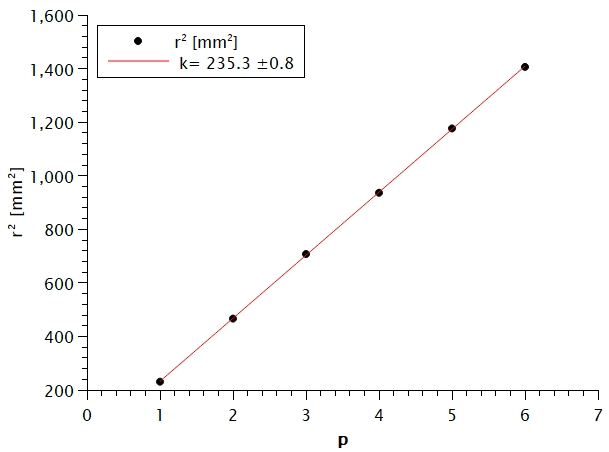
\includegraphics[width=0.9\linewidth]{fit}
			\caption{Závislost kvadrátu poloměru kroužku na jeho pořadí}
			\label{fig:mereni}
		\end{figure}
		Z experimentální tabulky se závislostí indukce na proudu v cívkách lze polynomickým fitem třetího stupně získat funkci indukce na proudu (obr. 2), se získanými koeficienty (funkcí) pracujeme pro získání velikosti magnetické indukce.
		\begin{figure}[H]
			\centering
			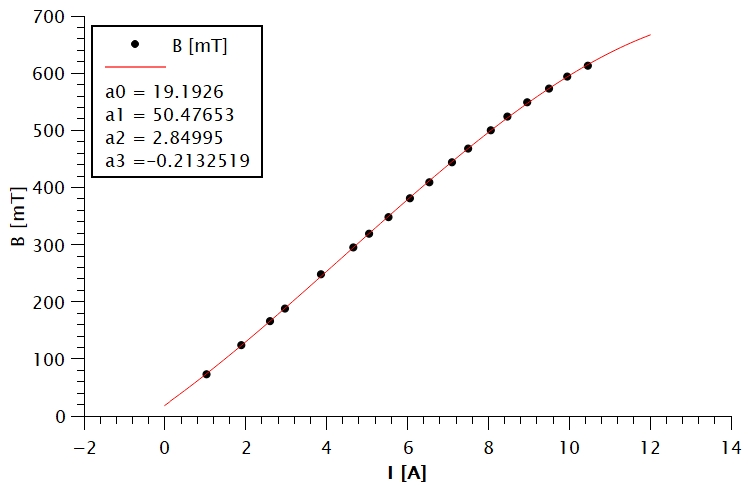
\includegraphics[width=0.9\linewidth]{indukce}
			\caption{Získané hodnoty závislosti velikosti magnetické indukce na proudu jejich proložení polynomem třetího stupně.}
			\label{fig:mereni}
		\end{figure}
		
		Pro hodnotu Bohrova magnetonu měříme poloměry kružnic a hodnotu získáváme použitím formule (4):\\
{\small 	\begin{tabular}{rlrr|ll}

	
		I [A] & B [mT] & $r_{a, p+1}$ &$ r_{b,p+1}$ & $\mu _\mathrm{B}^{ab}\mathrm{[A.m^2]}$ &$ \mu _\mathrm{B}^{bc} .10^{-24} \mathrm{[A.m^2]}$\\ \hline
		5.08 & 321 & 17.3 & 23.0 &$ 10.8\pm0.7 $&$ 9.7\pm0.8 $\\
		6.03 & 380 & 17.5 & 23.1 & $11.0\pm0.7 $&$ 9.4\pm0.7 $\\
		6.54 & 412 & 17.5 & 23.2 &$ 10.2\pm0.6 $&$ 9.8\pm0.7 $\\
		7.25 & 454 & 17.7 & 23.3 &$ 10.8\pm0.7 $&$ 9.9\pm0.7 $\\
		7.60 & 474 & 17.8 & 23.4 &$ 11.0\pm0.7 $&$ 10.4\pm0.8 $\\
		7.77 & 483 & 17.8 & 23.4 &$ 10.8\pm0.7 $&$ 10.2\pm0.8 $\\
		8.02 & 497 & 17.8 & 23.4 &$ 10.5\pm0.7 $&$ 9.9\pm0.8 $\\
		8.62 & 530 & 17.9 & 23.5 &$ 10.5\pm0.8 $&$ 10.2\pm0.8 $\\
		9.09 & 550 & 18.0 & 23.6 &$ 10.7\pm0.8 $&$ 10.6\pm0.9 $\\
		9.60 & 580 & 18.0 & 23.6 &$ 10.2\pm0.8 $&$ 10.1\pm0.9 $\\
		10.02 & 600 & 18.1 & 23.7 &$ 10.5\pm0.9 $&$ 10.6\pm0.9$ \\\hline \hline
			&		&		&	&$10.6 \pm 0.7$&$10.1\pm 0.8$\\
			

	\end{tabular}}
		Pozorujeme, že při kalkulaci z druhého a třetího setu (bc) získáváme lepší výsledky, než v případě setu prvního a druhého (ab). Takové výsledky jsme očekávali, jelikož pro větší kružnice bylo určení jejich poloměru jednodušší, než u kružnic menších. Hodnoty $r_a, r_b, r_c$ jsou ve všech případech stejné - na ně magnetická indukce nepůsobí, proto jsme pro každou z hodnot statisticky zpracovali hodnotu průměrnou a s ní pracovali pro všechny hodnoty proudu, resp. indukce:
		\begin{equation*}
			r_{a,p} = 16.22 \pm 0.05, \quad r_{b,p} = 22.3 \pm 0.05, \quad r_{c,p} = 27 \pm 0.05 \,\mathrm{mm}
		\end{equation*}
		Též lze spočítat rozdíl energie dvou blízkých spektrálních čar, tj. hlavních a vedlejších, a za pomocí formule (1) vykreslit závislost $\Delta E$ na $B$ (Obr. 3)a následně hodnotu Bohrova magnetonu určit.
		
		\begin{figure}[H]
			\centering
			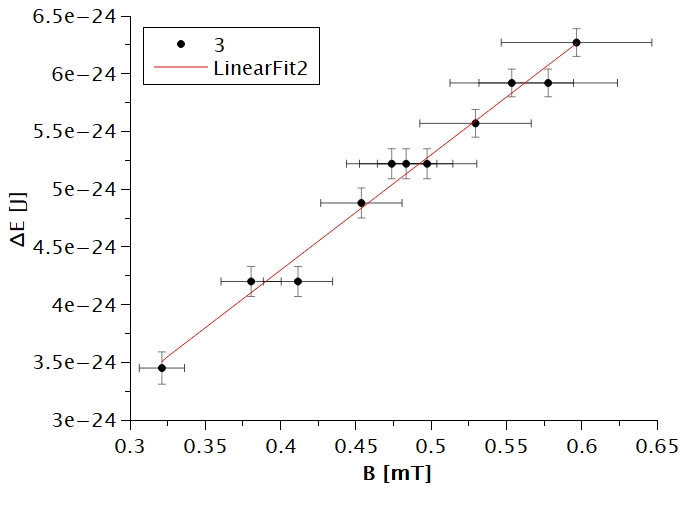
\includegraphics[width=0.8\linewidth]{Graph3}
			\caption[Závislost E na B]{}
			\label{fig:graph3}
		\end{figure}
		
		Tímto složitějším způsobem získáváme hodnotu Bohrova magnetonu:\\ $\mu_\mathrm{B} = 10.13 \pm 0.32 \cdot 10^{-24}\,\rm A.m^2$
		
		 
		Anomální Zeemanův jev pozorujeme úspěšně, vzniká 9 čar.\\
		V případě pozorování jevu kolmo na magnetickou indukci pozorujeme lineární polarizaci hlavní spektrální čáry i čar vedlejších. Při vertikální polarizaci (kolmo na magnetickou indukci) jsou přítomny pouze čáry vedlejší, hlavní je naopak přítomna při polarizaci horizontální ($\pm 90^\circ$, rovnoběžně s magnetickou indukcí). Při pozorování jevu rovnoběžně na magnetickou indukci není hlavní spektrální čára vyzářena vůbec, vedlejší čáry na lineární polarizátor nereagují - jsou totiž polarizovány kruhově, což dokazujeme vložením čtvrtvlnné destičky před lineární polarizátor, přičemž je polarizace vnitřního kroužku na vnější kolmá. Světlo lze nyní při správném nastavení polarizátoru vyfiltrovat, což svědčí o původně kruhové polarizaci, přičemž je u jedné složky pravotočivá a u druhé levotočivá. 
		
		\section{Závěr}
		Podařilo se nám ověřit funkčnost FP interferometru a následným zpracováním dat z něj stanovit velikost Bohrova magnetonu. Jak již je nastíněno v bezprostřední evaluaci výsledků po tabulce s daty, limitem přesnosti bylo samotné rozlišení CCD kamery - poloměry nám vycházely při malém proudovém rozdílu na pixel identické. Předpokládáme, že by vyšší rozlišení kamery mohlo přinést i větší přesnost experimentu (i samotná velikost nejistoty je ovlivněna zejména přesností "měřítka", kterým byla právě kamera). Ke skutečné hodnotě$^{[1]}$ je náš výsledek nicméně velice blízko, v rámci stanovené odchylky.. Úspěšně jsme stanovili polarizační stavy pro klasický Zeemanův jev.
		
		\section{Zdroje}
		1. The NIST Reference on Constants, Units and Uncertainty; Bohr Magneton.\\ Dostupné z WWW:\\ https://physics.nist.gov/cgi-bin/cuu/Value?mub
		
		
		
		% Nakonec nezapomeňte projet text programem vlna nebo vlnka, např.
		% 	vlna -m -l -n mojeuloha.tex
		% nebo zkontrolovat a opravit jednopísmenné předložky na koncích řádků ručně.
	\end{multicols}
\end{document}
